\chapter{Prosenttilaskenta}

Sana prosentti tulee latinan kielen sanoista pro centum, mikä tarkoittaa kirjaimellisesti sataa kohden. Prosentteja käytetään ilmaisemaan suhteellista osuutta. Prosentin merkki on \%.


\laatikko{1 prosentti $= 1\ \% = \frac{1}{100} = 0,01$}

\begin{esimerkki}
\mbox{}
\begin{itemize}
	\item $6 \ \% = \frac{6}{100} = 0,06$
	\item $48,2 \ \% = \frac{48,2}{100} = 0,482$
	\item $140 \ \% = \frac{140}{100} = 1,40$
\end{itemize}
\end{esimerkki}

\todo{tehtävä: ilmaise desimaalilukuna seuraavat prosentit}

%%%%PERUSARVO%%%%%%%
\laatikko{
Lukua, josta suhde lasketaan, kutsutaan \emph{perusarvoksi}.
}


\begin{esimerkki}
Jos sadan euron hintaisen tuotteen hintaa on alennettu 25 prosenttia, niin alennettu hinta on 75 euroa. Jos sen sijaan alkuperäinen hinta nousee 15 prosenttia, niin tuotteen uusi hinta on 115 euroa. Perusarvo on molemmissa tapauksissa 100 euroa.

\missingfigure{kuva suorakaiteesta, joka kuvaa perusarvoa (se voi olla vaik 10x10 pientä laatikkoa. Sit kuva, jossa peruarvosta on vähennetty 25~\% perusarvosta, eli 75 laatikkoa. Sit kuva, jossa perusarvoon on lisätty 15~\%, eli 115 laatikkoa. Sit sopivat havainnollistavat väritykset}
\end{esimerkki}


\todo{tehtävä perusarvosta}


%MUUTOSPROSENTTITEORIA
\laatikko{
Prosentteja käytetään usein ilmaisemaan suureiden muutoksia, esimerkiksi luku $b$ kasvaa luvuksi $a$. \emph{Muutosprosenttia} laskettaessa muutoksen suuruutta verrataan alkuperäiseen lukuun. Perusarvona on siis alkuperäinen arvo, johon nähden muutos on tapahtunut.

Jos kysytään, kuinka monta prosenttia $a$ on isompi $b$:tä, se tarkoittaa samaa, kuin kuinka monta $b$:n sadasosaa on se määrä, jolla $a$ on suurempi $b$:tä. Toisin sanoen kuinka monta $b$:n sadasosaa mahtuu $a-b$:hen. Se saadaan laskemalla

\begin{equation*}
\frac{a-b}{\frac{b}{100}} = \frac{a-b}{b} \cdot 100
\end{equation*}

Samalla tavalla saadaan laskettua, kuinka monta prosenttia luku kasvoi, kun se muuttui $a$:sta $b$:hen.
}




%TÄMÄ ON MUUTOSPROSENTTITEHTÄVÄESIMERKKI
\begin{esimerkki}
Vesan paino on tammikuussa 68 kg ja kesäkuussa 64 kg. Kuinka monta prosenttia Vesa on laihtunut?

\textbf{Ratkaisu.}

Lasketaan 
\begin{equation*}
\frac{68-64}{68} = \frac{4}{68}=0,06 = 6\ \%
\end{equation*}

\textbf{Vastaus.}

Vesa on laihtunut $6\ \%$.
\end{esimerkki}

\begin{tehtava}

Oppikirjamaraton-tiimi kävi lounastamassa. Osoita oheisen kuitin tiedoilla vääräksi yleinen virhekäsitys, että 13 \%:n arvonlisävero olisi 13~\% lopullisesta myyntihinnasta.
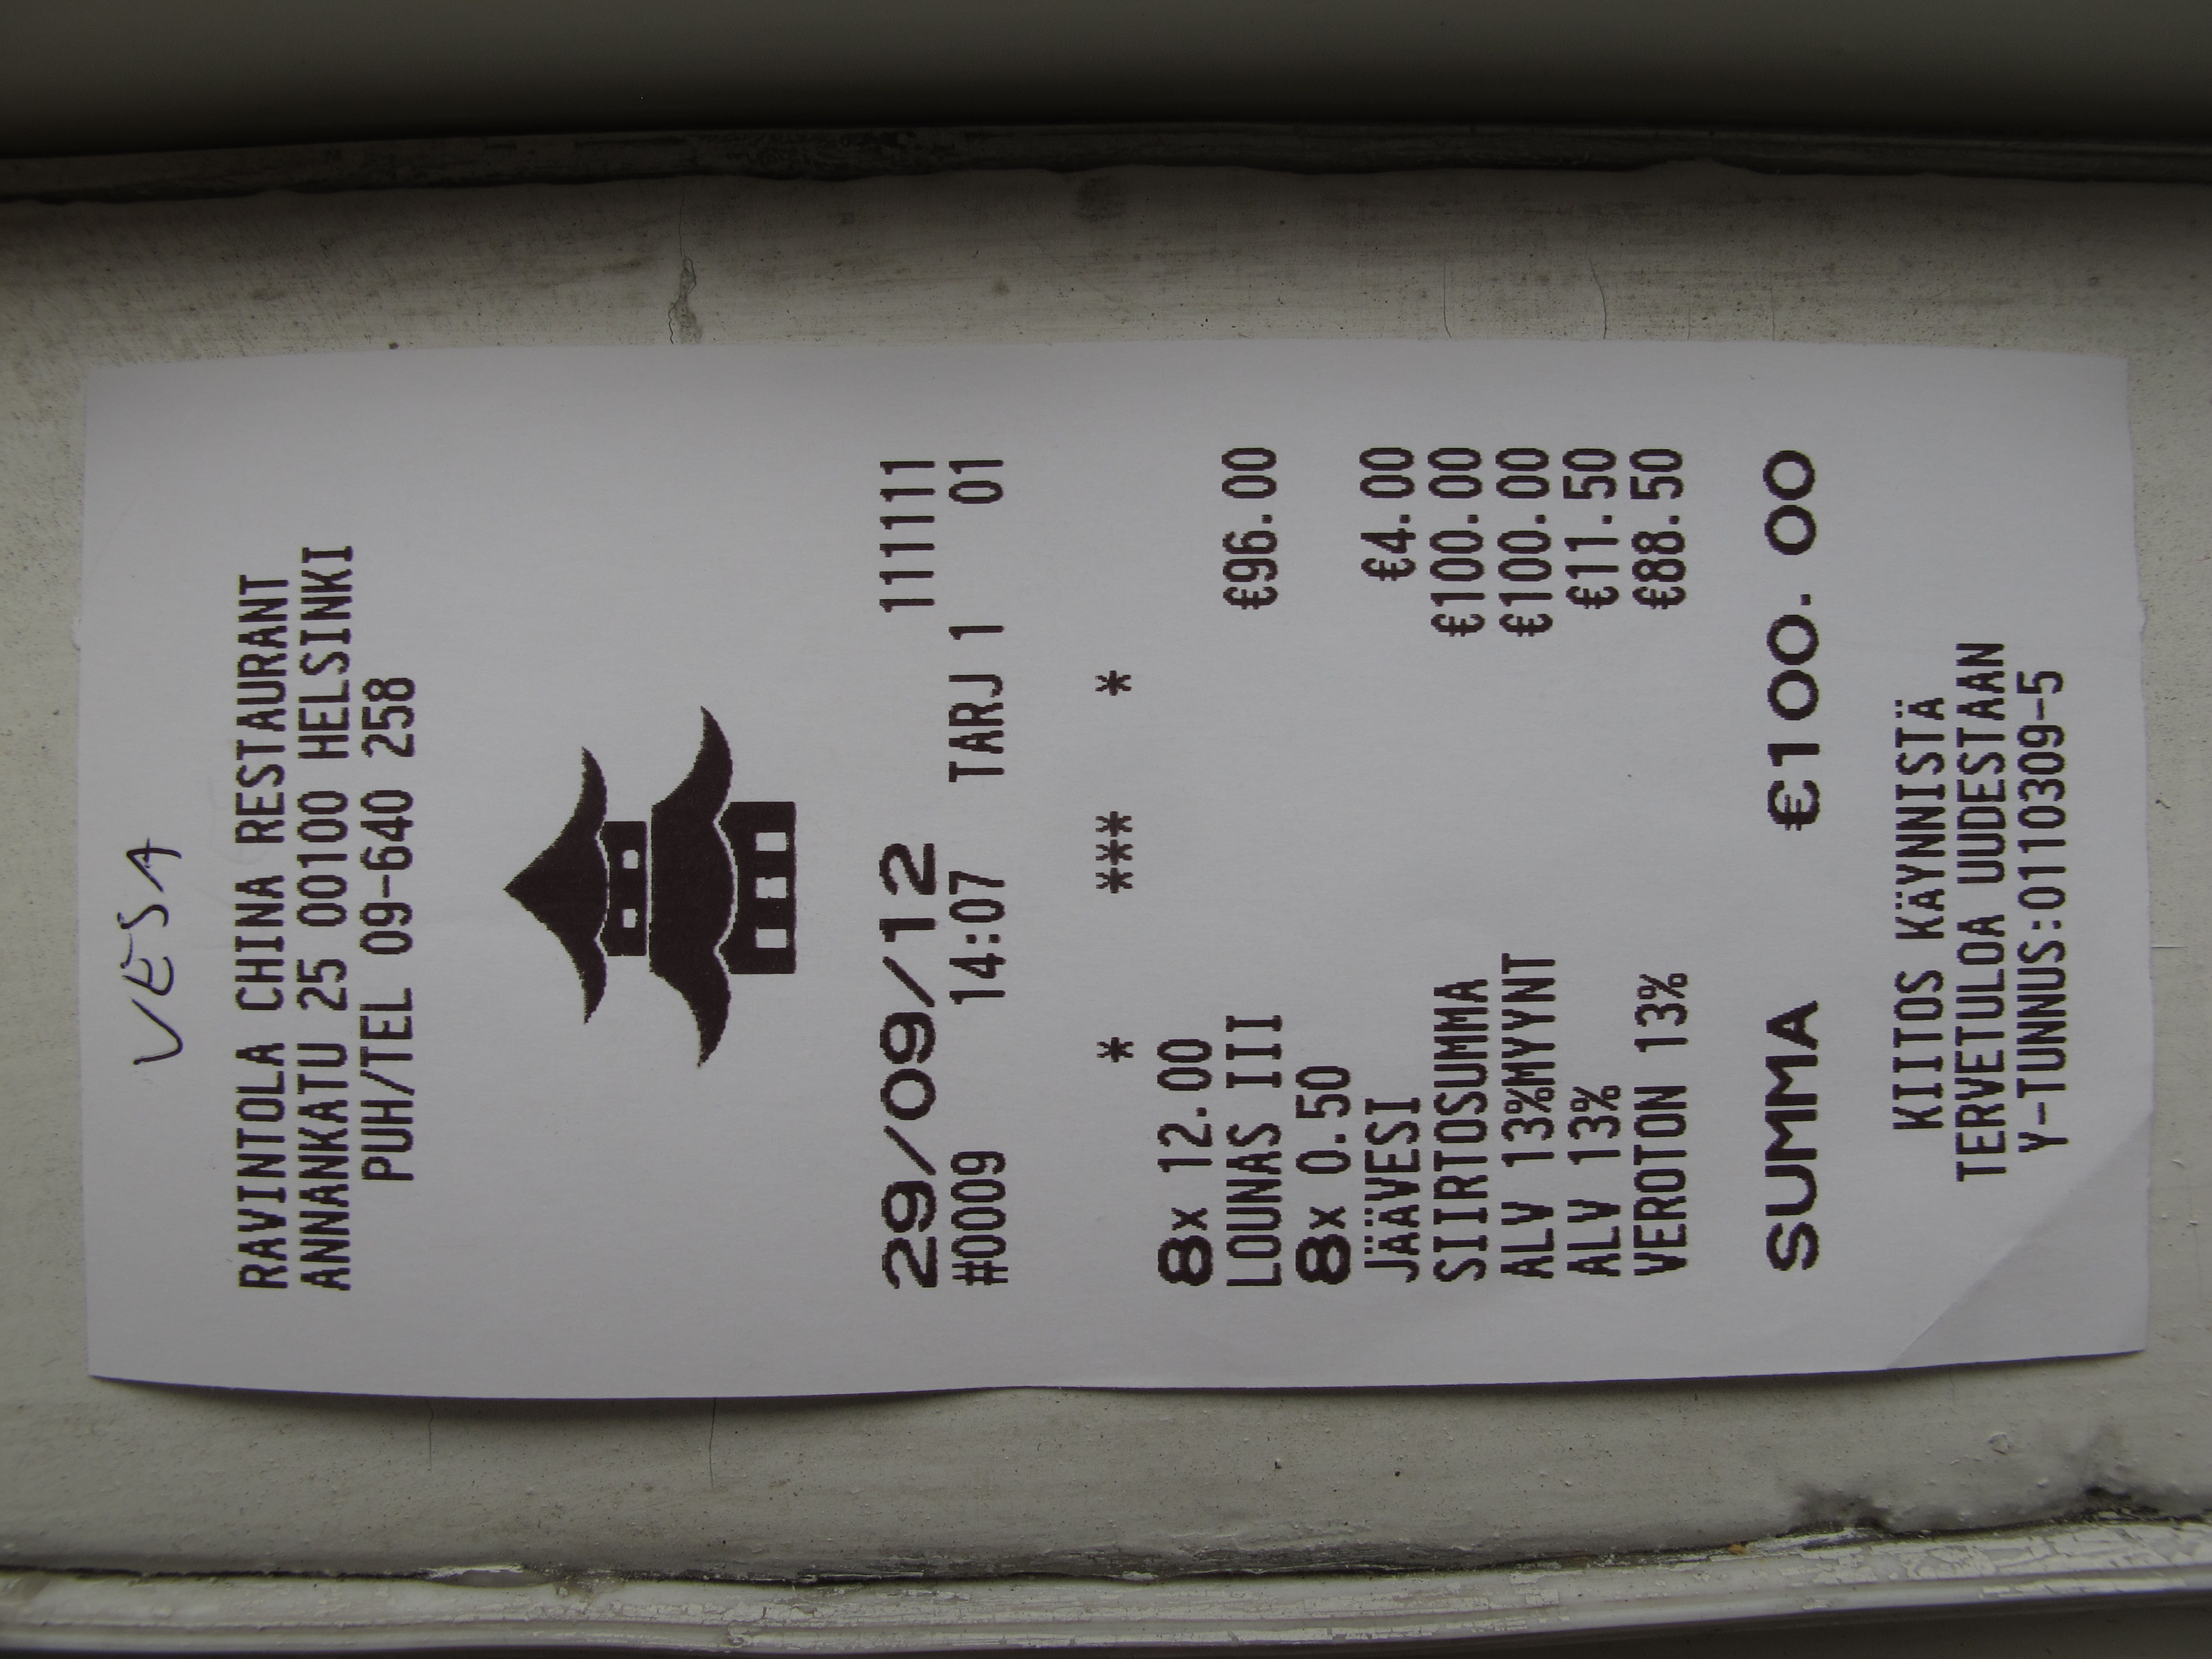
\includegraphics[width=80mm, angle=270]{02-yhtalot/kuvia/alv-kuitti}

\begin{vastaus}
13 \% sadasta eurosta on 13 euroa, ei 11,50 euroa, niin kuin kuitissa todetaan.
\end{vastaus}


\end{tehtava}


%%%VERTAILUPROSENTTI%%%%%
\laatikko{
\emph{Vertailuprosentilla} ilmaistaan, kuinka monta prosenttia luku on jostain toisesta luvusta. Vertailuprosentin laskennassa käytetään perusarvona sitä lukua, johon verrataan.

Jos kysytään, kuinka monta prosenttia $b$ on $a$:stä, se tarkoittaa samaa, kuin kuinka monta $a$:n sadasosaa $b$ on. Toisin sanoen kuinka monta $a$:n sadasosaa $b$:hen mahtuu. Se saadaan laskemalla 

\begin{equation*}
\frac{b}{\frac{a}{100}} = \frac{b}{a} \cdot 100
\end{equation*}

\missingfigure{havainnollistava kuva vertailuprosentista suorakulmioiden avulla}
}

%TÄMÄ ON VERTAILUPROSENTTITEHTÄVÄESIMERKKI
\begin{esimerkki}
Vesa ansaitsee kuukaudessa ${2\,300}$ euroa ja Antero ${1\,700}$ euroa. Kuinka monta prosenttia Anteron tulot ovat Vesan tuloista? 

\textbf{Ratkaisu.}

Lasketaan

\begin{equation*}
\frac{1700}{2300}  \approx 0,74 = 74 \  \%.
\end{equation*}

Laskuissa käytettävä perusarvo on Vesan palkka eli 2300 euroa.
    
\textbf{Vastaus.}

$74~\%$
\end{esimerkki}



%%%%PROSENTTIYKSIKKÖ
\laatikko{
\emph{Prosenttiyksikkö} mittaa prosenttiosuuksien välisiä eroja. Esimerkiksi $4\ \%$ on $2$ prosenttiyksikköä suurempi kuin $2\ \%$, mutta $100\ \%$ suurempi kuin $2\ \%$. Jos prosenttiluku muuttuu, muutos voidaan ilmaista joko prosentteina tai prosenttiyksikköinä.
}


%%%%%%PROSENTTIYKSIKKÖTEHTÄVÄESIMERKKI
\begin{esimerkki}
    Tuotteen markkinaosuus on vuoden tammikuussa 10~\% ja kesäkuussa 15~\%. 
    \begin{enumerate}[a)]
    \item Kuinka monta prosenttia tuotteen markkinaosuus on noussut?
    
    \item Kuinka monta prosenttiyksikköä tuotteen markkinaosuus on noussut?
    \end{enumerate}
    
    {\bf Ratkaisu.} 
    
    \begin{enumerate}[a)]
    \item Tuotteen markkinaosuus on noussut
    \[
    \frac{15-10}{10} = \frac{5}{10} = 50\ \%.
    \]
    
    \item Tuotteen markkinaosuus on noussut $15-10=5$ prosenttiyksikköä. 
    \end{enumerate}
    
    {\bf Vastaus.}
    
    \begin{enumerate}[a)]
    \item 50 prosenttia
    \item 5 prosenttiyksikköä.
    \end{enumerate}
\end{esimerkki}

\section*{Tehtäviä}

\begin{tehtava}
    Laukun normaalihinta on 225 euroa, ja se on 25~\%:n alennuksessa.
    Mikä on alennettu hinta?
    \begin{vastaus}
    Vastaus: 168,75 euroa
    \end{vastaus}
\end{tehtava}

\begin{tehtava}
    Jaakon kuukausipalkka on 1623,52 euroa. Hän saa 1,3~\% palkankorotuksen.
    Mikä on Jaakon kuukausipalkka korotuksen jälkeen?
    \begin{vastaus}
    1644,63 euroa
    \end{vastaus}
\end{tehtava}

\begin{tehtava}
    Kirjan myyntihinta, joka sisältää arvolisäveron, on 9~\% suurempi kuin kirjan veroton hinta. Laske kirjan veroton hinta, kun myyntihinta on 27 \euro.
    \begin{vastaus}
        Vastaus: Kirjan veroton hinta on 24,77 \euro.
    \end{vastaus}
\end{tehtava}

\begin{tehtava}
	Sokerijuurikkaassa on 18~\% sokeria. Kuinka paljon sokerijuurikkaita tarvitaan valmistettaessa 8 tonnia sokeriliuosta, jonka sokeripitoisuus on 4,5~\%?
	\begin{vastaus}
        Vastaus: 2 tonnia
    \end{vastaus}
\end{tehtava}

\begin{tehtava}
    Perussuomalaisten kannatus oli vuoden 2007 eduskuntavaaleissa 4,1~\% ja 
    vuoden 2011 eduskuntavaaleissa 19,1~\%. Kuinka monta prosenttiyksikköä 
    kannatus nousi? Kuinka monta prosenttia kannatus nousi?
    \begin{vastaus}
    Vastaus: Kannatus nousi 15 prosenttiyksikköä. Prosentteina mitattuna kannatus nousi 366~\%.
    \end{vastaus}
\end{tehtava}

\begin{tehtava}
    Askartelukaupassa on alennusviikot, ja kaikki tavarat myydään 60~\%:n 
    alennuksella. Viimeisenä päivänä kaikista hinnoista annetaan vielä 
    lisäalennus, joka lasketaan aiemmin alennetusta hinnasta. Minkä suuruinen 
    lisäalennus tulee antaa, jos lopullisen kokonaisalennuksen halutaan olevan 80~\%?
    \begin{vastaus}
        Vastaus: 50~\%.
    \end{vastaus}
\end{tehtava}

\begin{tehtava}
	Hedelmissä on vettä aluksi 60~\%. Kuinka monta prosenttia vedestä on 
	haihdutettava, jotta hedelmissä tämän jälkeen olisi vain 20~\% vettä?
	\begin{vastaus}
		Vastaus: 50~\%.
	\end{vastaus}
\end{tehtava}

\begin{tehtava}
    Erään pankin myöntämä opintolaina kasvaa korkoa 2~\% vuodessa. Kuinka monta 
    prosenttia laina on kasvanut korkoa alkuperäiseen verrattuna kymmenen vuoden kuluttua?
    \begin{vastaus}
        Vastaus: 22~\%.
    \end{vastaus}
\end{tehtava}

\begin{tehtava}

Samulin pituus on 165 cm ja Joonaksen 173 cm.
\begin{enumerate}
\item Kuinka monta prosenttia Samulin pituus on Joonaksen pituudesta?
\item Kuinka monta prosenttia Samuli on lyhyempi kuin Joonas?
\item Kuinka monta prosenttia Joonas on pidempi kuin Samuli?
\end{enumerate}

\begin{vastaus}
\begin{enumerate}
\item 95,4~\%
\item 4,62~\%
\item 4,85~\%
\end{enumerate}
\end{vastaus}

\end{tehtava}

\begin{tehtava}
	Yleinen arvonlisäveroprosentti oli Suomessa vuonna 2012 23~\% tuotteen verottomasta 
	hinnasta. Tuotteen hinta koostuu sen verottomasta hinnasta 
	ja tuotteesta maksettavasta arvonlisäverosta. Kuinka monta 
	prosenttia arvonlisävero on tuotteen myyntihinnasta?
	\begin{vastaus}
		18,7~\%
	\end{vastaus}
\end{tehtava}

\begin{tehtava}
	Kun matkalipun hintaa korotettiin 10,0~\%, matkustajien määrä väheni 10,0~\%. 
	Kuinka monella prosentilla tällöin lisääntyivät tai vähentyivät liikennöitsijän 
	lipputulot?
	\begin{vastaus}
		Vähentyvät 1 prosentilla.
	\end{vastaus}
\end{tehtava}
%Ansiotuloverotus on Suomessa progressiivista: suuremmista tuloista maksetaan

\begin{tehtava}
    Tuoreissa omenissa on vettä 80~\% ja sokeria 4~\%. Kuinka monta prosenttia sokeria on samoissa omenissa, kun ne on kuivattu siten, että kosteusprosentti on 20? [K2000, 4]
    \begin{vastaus}
        Vastaus: 16~\%
    \end{vastaus}
\end{tehtava}

\begin{tehtava}
    Kappaleen putoamisen kesto maahan korkeudelta $x$ on kääntäen verrannollinen putoamiskiihtyvyyden $g$ neliöjuureen. Vakio $g$ on kullekin taivaankappaleelle ominainen ja eri puolilla taivaankappaletta likimain sama. Empire State Buildingin katolta (korkeus $381$ m) pudotetulla kuulalla kestää n. $6,2$ s osua maahan. Marsin putoamiskiihtyvyys on $37,6$ \% Maan putoamiskiihtyvyydestä. 
    
    Jos Empire State Building sijaitsisi Marsissa, kuinka monta prosenttia pitempi aika kuluisi kuulan maahan osumiseen?
    \begin{vastaus}
        Vastaus: $10$ s
    \end{vastaus}
\end{tehtava}

\begin{tehtava}
Matin ja Iidan duo saa julkisuutta, ja he alkavat myydä CD-levyään keikkojen yhteydessä 10 euron kappalehinnalla. Jonkin ajan päästä he päättävät laskea CD:n hintaa 20 prosenttia. Matti alkaa kuitenkin katua päätöstä, ja ehdottaa tämän alennetun hinnan korottamista 20 prosentilla. Mikä olisi tämän toimenpiteen jälkeen CD:n uusi hinta? Montako prosenttia olisi korotuksen oltava, jotta oikeasti päästäisiin takaisin alkuperäiseen 10 euron hintaan?
    \begin{vastaus}
25~\%
    \end{vastaus}
\end{tehtava}

\begin{tehtava}
Jalkapalloilija Georgios Samaras teki ensimmäisellä kaudellaan Skotlannin valioliigassa (2007-08) 5 maalia Celtic F.C.:n paidassa. Seuraavalla kaudella Samaras teki Celticille liigassa 15 maalia. Kuinka monta prosenttia Samaraksen maalimäärä nousi?
    \begin{vastaus}
200~\%
    \end{vastaus}
\end{tehtava}

\begin{tehtava}
 Kaupungissa tuli jokaisen talonomistajan suorittaa kaupungin kassaan 5~\% saadusta hyyrymäärästä\footnote{vuokra, ruotsin sanasta \emph{hyra}}. Sittemmin määrättiin, että mainittu prosentti oli oleva 10. Monellako prosentilla täytyy talonomistajien korottaa hyyryjä saadakseen saman puhtaan säästön kuin ennen? [YO 1877, 4]
    \begin{vastaus}
5,6~\%
    \end{vastaus}
\end{tehtava}
